\FloatBarrier
\section{Official GarlTTC benchmark result}
\label{sec:official}

\subsection{Public ranking and bandwise accuracy}

As of 28 October 2026, PHASE-TTC ranks first among the three displayed submissions on the official GarlTTC Test leaderboard. Submission \OfficialPhaseSubmissionID{}, listed as \emph{PHASE-TTC (TRAIN40, 650 ms causal history)}, records Overall MiD \OfficialPhasePublishedOverallMiD{} over \OfficialSampleCount{} scored tokens with a 0\% scorer-defined failure rate. The next displayed score is \OfficialGarlOverallMiD{} for the Garl-TTC reference. \citep{codabench2026} \evidence{B01}

The scorer returns Overall MiD \OfficialPhaseOverallMiD{} at full precision, consistent with the rounded public entry. Relative to Garl-TTC's published \OfficialGarlOverallMiD{}, PHASE-TTC reduces the ranking metric by \OfficialOverallRelativeGain{}. All four TTC bands improve (Table~\ref{tab:official-benchmark}); the large positive-TTC band has the largest relative reduction and the negative band the smallest. Percentage reductions combine the unrounded PHASE-TTC values with Garl-TTC's published two-decimal scores. \evidence{B01,B02}

\begin{table}[H]
\centering\small
\caption{Official GarlTTC Test scores on 28 October 2026 (lower is better). PHASE-TTC scores are shown to four decimals and Garl-TTC at published precision. Relative reductions use unrounded PHASE-TTC scores. Both entries have 6,762 scored tokens and 0\% scorer-defined failures. \evidence{B01,B02}}
\label{tab:official-benchmark}
\begin{tabular}{lrrr}
\toprule
\textbf{Metric} & \textbf{PHASE-TTC} & \textbf{Garl-TTC} & \textbf{Decrease} \\
\midrule
Overall & 35.8015 & 45.03 & 20.49\% \\
Crucial & 43.5190 & 53.13 & 18.09\% \\
Small & 28.2568 & 37.58 & 24.81\% \\
Large & 25.7179 & 40.61 & 36.67\% \\
Negative & 29.9314 & 31.29 & 4.34\% \\
\bottomrule
\end{tabular}
\end{table}


\subsection{Where the weighted difference comes from}

For band $b$, the additive contribution is $w_b(\mathrm{MiD}^{\mathrm{Garl}}_b-\mathrm{MiD}^{\mathrm{PHASE}}_b)$. The crucial and small bands contribute \OfficialCrucialSmallContributionShare{} of the Overall difference under weights 0.5 and 0.3. The large band's 0.1 weight limits its contribution despite its larger relative reduction; the negative band contributes least.



\begin{figure}[H]
\centering
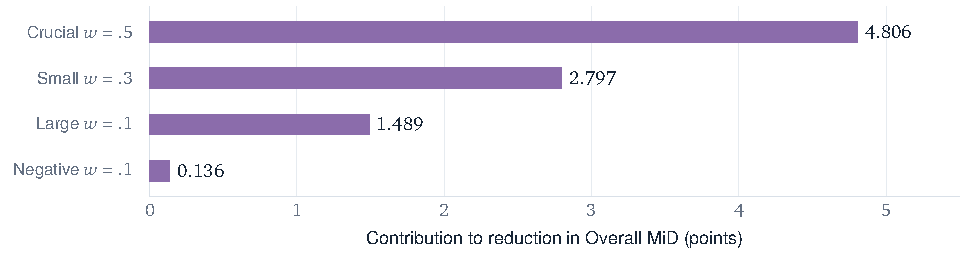
\includegraphics[width=.92\linewidth]{figures/rev_weighted.pdf}
\caption{\textbf{Bandwise contributions to the Overall MiD difference.} Crucial and small TTC account for about 82\% under the benchmark's $0.5/0.3/0.1/0.1$ weights. Table~\ref{tab:official-weighted-contributions} gives the rounding reconciliation. \evidence{B01,B02}}
\label{fig:official-weighted-contributions}
\end{figure}

\subsection{Metric and evaluation population}

The four TTC bands cover $(0,3]$, $(3,6]$, $(6,10]$, and $(-10,0]$ seconds. MiD measures error in the motion-in-depth coordinate defined in Section~\ref{sec:protocol}. The ranking uses the weighted Overall MiD; the scorer also reports \texttt{mean\_MiD}, an unweighted average over finite per-query errors. \citep{garlscorer2026}

The \OfficialSampleCount{} scored tokens represent 5,805 distinct physical queries and 957 aliases in the submitted package. Aliases reuse predictions at the same sensor query. The official failure criterion marks nonfinite TTC predictions or predictions with $|\widehat T|<0.1$\,s. Band scores average finite MiD values. The available aggregate outputs support bandwise analysis; studying individual errors requires per-query scores. \evidence{L44,B02}

\subsection{Scope of the comparison}

The submission declares RGB and event inputs, TRAIN40 fitting, and up to 650\,ms of causal history. Because the evaluator scores submitted TTC values, the leaderboard compares complete systems with their own temporal support, localization, supervision, and runtime choices. Section~\ref{sec:design-analysis} examines modality and temporal dependencies within the tested development configurations.

The official result measures the submitted system on private test targets. The exploratory EvTTC transfer compares frozen routes on development-exposed, positive-TTC sequences with annotated object regions. Section~\ref{sec:runtime} evaluates execution time separately, including deadline misses.
\FloatBarrier
